\documentclass[spanish,letterpaper,oneside]{article}

% Datos del documento
\def\documenttitle {Lenguaje algebraico y perímetros}
\def\documentsubtitle {Temas selectos de matemáticas I}
\def\documentsubject {Actividad 9 · Ficha de trabajo y propuesta didáctica}
\def\documentauthor {Mtro. Martín Jonathan de la Cruz Muñoz}
\def\coursename {Temas selectos de matemáticas I}
\def\coursecode {PFM02}

% Identidad institucional
\def\universityname {Instituto de Investigación, Innovación y Estudios de Posgrado para la Educación del Estado de Nuevo León}
\def\universityfaculty {Maestría en Aprendizaje y Enseñanza de las Matemáticas}
\def\universitydepartment {Temas selectos de matemáticas I}
\def\universitydepartmentimage {img/iiiepe/marca-iiiepe.png}
\def\universitydepartmentimagecfg {height=1.75cm}
\def\universitylocation {Monterrey, Nuevo León}
\def\studentfullname {Mtro. Martín Jonathan de la Cruz Muñoz}
\def\studentid {00874}
\def\studentemail {martin.delacruz@campus.iiiepe.edu.mx}
\def\programperiod {1er tetramestre, marzo--julio de 2026}
\def\programmodality {Modalidad presencial}
\def\programshort {MAEM}

\def\authortable {
  \begin{tabular}{ll}
    \textbf{Alumno:} & \studentfullname \\
    Matrícula: & \studentid \\
    Correo institucional: & \studentemail \\
    Unidad: & \coursename \\
    Programa: & \programshort \\
    Periodo: & \programperiod \\
    & \\
    \multicolumn{2}{l}{Fecha de realización: 13 de octubre de 2026} \\
    \multicolumn{2}{l}{\universitylocation}
  \end{tabular}
}

\input{template}

\usepackage{helvet}
\renewcommand{\familydefault}{\sfdefault}
\usepackage{array}
\usepackage{longtable}
\usepackage{pdflscape}
\usepackage{tikz}
\usepackage[most]{tcolorbox}
\usetikzlibrary{arrows.meta,positioning,calc,fit,backgrounds}

\definecolor{iiiepeNavy}{HTML}{163B5C}
\definecolor{iiiepeBlue}{HTML}{1F6F9F}
\definecolor{iiiepeAqua}{HTML}{20B7A8}
\definecolor{iiiepeOrange}{HTML}{F28C28}
\definecolor{iiiepePaper}{HTML}{F6F8F7}
\definecolor{iiiepeInk}{HTML}{1E2A32}
\def\portraittitlecolor {iiiepeNavy}
\setcitestyle{authoryear,open={(},close={)}}

\newcommand{\insertcoverwatermark}{%
  \AddToShipoutPictureBG*{%
    \begin{tikzpicture}[remember picture,overlay]
      \node[opacity=.09,inner sep=0pt] at (current page.center)
      {\includegraphics[width=.58\paperwidth]{img/iiiepe/logo-puntos.png}};
    \end{tikzpicture}%
  }%
}

\newtcolorbox{reportelecturabox}[1][]{%
  enhanced,breakable,
  colback=iiiepePaper,colframe=iiiepeNavy,
  boxrule=1pt,leftrule=4pt,arc=2pt,
  left=8pt,right=8pt,top=6pt,bottom=6pt,
  before skip=6pt,after skip=10pt,
  fonttitle=\bfseries\color{white},coltitle=white,
  colbacktitle=iiiepeNavy,
  attach boxed title to top left={xshift=8pt,yshift=-2pt},
  boxed title style={colback=iiiepeNavy,colframe=iiiepeNavy,arc=1pt},
  title={Reporte de lectura},#1}

\newtcolorbox{fichalecturabox}[1][]{%
  enhanced,breakable,
  colback=iiiepeAqua!7,colframe=iiiepeAqua!70!iiiepeNavy,
  boxrule=.6pt,arc=1pt,
  left=7pt,right=7pt,top=4pt,bottom=4pt,
  fontupper=\small,before upper={\setstretch{1.0}},
  fonttitle=\bfseries\color{iiiepeNavy},coltitle=iiiepeNavy,
  colbacktitle=iiiepeAqua!7,
  title={Ficha de la lectura},#1}



\usepackage{tabularx,colortbl,pgfplots,enumitem,needspace}\pgfplotsset{compat=1.18}\definecolor{iiiepePale}{HTML}{EEF5F8}
\setlength{\parskip}{5pt}\setlength{\parindent}{0pt}
\begin{document}\insertcoverwatermark\templatePortrait\templatePagecfg\templateFinalcfg\fancyfoot{}\fancyfoot[L]{\scriptsize IIIEPE · MAEM}\fancyfoot[C]{\scriptsize\thepage}\fancyfoot[R]{\scriptsize Actividad 9}\setstretch{1.3}\raggedbottom
\section{Lenguaje común, símbolos y significado}
El álgebra permite expresar relaciones que permanecen válidas para distintas cantidades. El contenido de la sesión incluye traducir situaciones al lenguaje algebraico y representar perímetros. La propuesta utiliza mantenimiento y diseño de piezas como contextos de transferencia, conservando el objetivo matemático de identificar variables, constantes y operaciones.
\section{Fase 1 · Recuperación de saberes}
Si una pieza rectangular tiene ancho $x$ y largo $x+3$, ¿cómo expresar el material necesario para su contorno? El dibujo permite distinguir el perímetro del área y cuestionar la respuesta incompleta $x(x+3)$, que representa una superficie.
\section{Fase 2 · Traducción e indagación}


{\small\setstretch{1.1}\renewcommand{\arraystretch}{1.25}
\begin{longtable}{|>{\raggedright\arraybackslash}p{\dimexpr0.5\linewidth-2\tabcolsep-2\arrayrulewidth\relax}|>{\raggedright\arraybackslash}p{\dimexpr0.5\linewidth-2\tabcolsep-2\arrayrulewidth\relax}|}\hline
\rowcolor{iiiepePale} \textbf{Expresión verbal} & \textbf{Modelo y condición} \\\hline
\endfirsthead
\hline
\rowcolor{iiiepePale} \textbf{Expresión verbal} & \textbf{Modelo y condición} \\\hline
\endhead
El triple de un número más cinco & $3x+5$ \\\hline
La tercera parte de la suma de un número y cinco & $(x+5)/3$ \\\hline
Dos números consecutivos & $n$ y $n+1$, con $n\in\mathbb{Z}$ \\\hline
El cuadrado de una diferencia & $(a-b)^2$ \\\hline
Una diferencia de cuadrados & $a^2-b^2$ \\\hline
Costo fijo de 250 pesos y 80 por hora & $C(h)=250+80h$, con $h\ge0$ \\\hline
\end{longtable}}


La lectura de paréntesis modifica el significado: $3(x+5)$ no equivale a $3x+5$. También debe distinguirse una expresión, que puede evaluarse, de una ecuación, que afirma igualdad y puede imponer una condición.
\section{Fase 3 · Perímetros resueltos}
Para el rectángulo de lados $x$ y $x+3$, $P=2x+2(x+3)=4x+6$. Si $x=5$ cm, $P=26$ cm. Para un triángulo de lados $x+1$, $x+2$ y $x+3$, $P=3x+6$. Si $x=4$, sus lados miden 5, 6 y 7 cm y cumplen la desigualdad triangular.
Un trapecio isósceles de bases $x+6$ y $x+2$ y lados iguales $x$ tiene $P=(x+6)+(x+2)+2x=4x+8$. Para que exista un trapecio no degenerado, cada lado debe superar la mitad de la diferencia de bases: $x>2$. Si $x=5$, $P=28$ cm. Un modelo geométrico requiere condiciones de existencia, además de una expresión correcta.
\begin{center}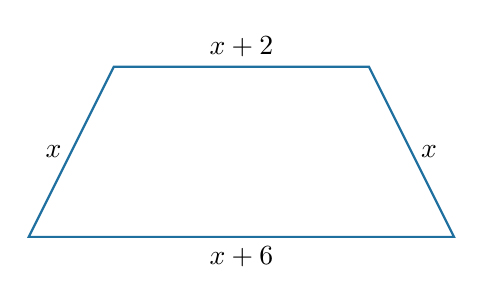
\begin{tikzpicture}[scale=.9]
\draw[thick,iiiepeBlue] (0,0)--(6,0)--(4.8,2.4)--(1.2,2.4)--cycle;
\node[below] at (3,0){$x+6$};\node[above] at (3,2.4){$x+2$};\node[left] at (.6,1.2){$x$};\node[right] at (5.4,1.2){$x$};
\end{tikzpicture}\end{center}
\section{Fase 4 · Comunicación y aplicación}
Con un costo fijo de 250 pesos y 80 por hora, cinco horas cuestan $C(5)=650$ pesos. Inversamente, si el presupuesto es 890, $250+80h=890$ conduce a $h=8$ horas. El modelo no incorpora refacciones ni impuestos: son supuestos explícitos del ejemplo. Se pide explicar qué representa cada término y cómo cambia el resultado si varía el costo fijo.
\section{El reto original y la generalización}
El recurso presenta una caja con la igualdad $\square+123=258$. Si la cantidad desconocida es $x$, restar 123 a ambos miembros da $x=135$. La comprobación $135+123=258$ confirma el resultado. La caja, la palabra ``número'' y la letra $x$ son representaciones de la misma cantidad desconocida.
Para generalizar el perímetro del rectángulo, una tabla con $x=1,2,3$ produce $P=10,14,18$; el aumento es 4 por cada unidad de $x$. El dibujo explica la razón: al crecer $x$ una unidad, aumentan las cuatro contribuciones del contorno. La expresión $P=4x+6$ representa todos los casos, mientras una tabla finita solo muestra algunos.
El caso del trapecio exige otra comprobación: la diferencia entre bases es 4 y el desplazamiento horizontal de cada lado es 2. Una longitud lateral $x=2$ generaría altura cero; por eso se requiere $x>2$. El lenguaje algebraico debe conservar las condiciones geométricas y no funcionar como manipulación desligada del objeto.
\section{Secuencia de aplicación y evaluación}
Traducir relaciones y justificar expresiones de perímetro. La duración propuesta es de 70 minutos, ajustable al diagnóstico y a los recursos. Esta planeación sigue la progresión de los recursos institucionales (IIIEPE, 2026); los tiempos y apoyos son decisiones de codiseño, no datos de una aplicación ya realizada.

{\small\setstretch{1.1}\renewcommand{\arraystretch}{1.25}
\begin{longtable}{|>{\raggedright\arraybackslash}p{\dimexpr0.23\linewidth-2\tabcolsep-2\arrayrulewidth\relax}|>{\raggedright\arraybackslash}p{\dimexpr0.49\linewidth-2\tabcolsep-2\arrayrulewidth\relax}|>{\raggedright\arraybackslash}p{\dimexpr0.28\linewidth-2\tabcolsep-2\arrayrulewidth\relax}|}\hline
\rowcolor{iiiepePale} \textbf{Fase y tiempo} & \textbf{Actividad y mediación} & \textbf{Evidencia} \\\hline
\endfirsthead
\hline
\rowcolor{iiiepePale} \textbf{Fase y tiempo} & \textbf{Actividad y mediación} & \textbf{Evidencia} \\\hline
\endhead
1. Reto y saberes (8 min) & Resolver la caja del recurso y representar la incógnita. & Predicción individual y pregunta. \\\hline
2. Plan de indagación (12 min) & Contrastar expresión, ecuación y significado de paréntesis. & Plan explicado y criterios. \\\hline
3. Construcción y análisis (25 min) & Modelar un perímetro con tabla, dibujo y expresión. & Registro o procedimiento trazable. \\\hline
4. Comunicación y aplicación (15 min) & Comprobar un valor y discutir una condición de existencia. & Argumento con comprobación. \\\hline
5. Metacognición (10 min) & Revisar una traducción ambigua y producir un problema equivalente. & Versión revisada y justificación. \\\hline
\end{longtable}}
\subsection{Criterios observables y retroalimentación}

{\small\setstretch{1.1}\renewcommand{\arraystretch}{1.25}
\begin{longtable}{|>{\raggedright\arraybackslash}p{\dimexpr0.22\linewidth-2\tabcolsep-2\arrayrulewidth\relax}|>{\raggedright\arraybackslash}p{\dimexpr0.4\linewidth-2\tabcolsep-2\arrayrulewidth\relax}|>{\raggedright\arraybackslash}p{\dimexpr0.38\linewidth-2\tabcolsep-2\arrayrulewidth\relax}|}\hline
\rowcolor{iiiepePale} \textbf{Criterio} & \textbf{Evidencia de logro} & \textbf{Acción si necesita apoyo} \\\hline
\endfirsthead
\hline
\rowcolor{iiiepePale} \textbf{Criterio} & \textbf{Evidencia de logro} & \textbf{Acción si necesita apoyo} \\\hline
\endhead
Traducción & Explica traducción con un caso de la actividad. & Pedir una representación concreta y contrastar dos casos. \\\hline
Variables y dominio & Conserva variables y dominio en el desarrollo y justifica sus pasos. & Modelar un paso, retirar gradualmente la ayuda y solicitar otro caso. \\\hline
Representaciones & Utiliza representaciones para contrastar una respuesta o representación. & Comparar la evidencia inicial y la corregida con una pregunta específica. \\\hline
Comprobación & Relaciona comprobación con la conclusión y un límite del problema. & Solicitar una comprobación independiente y un caso de transferencia. \\\hline
\end{longtable}}
El instrumento es una propuesta docente. Cada criterio se registra como logrado con autonomía, logrado con apoyo o aún no demostrado; no se asigna una calificación observada sin aplicar la actividad. En la coevaluación, un compañero verifica un criterio y formula una pregunta; en la autoevaluación, el estudiante explica una corrección; el docente contrasta ambas evidencias y decide el siguiente apoyo.\subsection{Participación y apoyos}
La inclusión se concreta en alternativas de representación y de acceso; el pensamiento crítico, en justificar y contrastar. Los roles de cálculo, registro y explicación se rotan para que todos produzcan una evidencia individual. Quien necesita apoyo dispone de un ejemplo parcial y preguntas graduadas; quien ya domina el procedimiento analiza un contraejemplo o cambia una condición. Estas acciones deben observarse durante la aplicación para valorar su funcionamiento.

\section{Fase 5 · Reflexión y evaluación}
Evaluaría tres evidencias: traducción verbal, representación geométrica y comprobación con un valor. Para apoyar a quien aún no generaliza, usaría una tabla con valores de $x$ y contornos dibujados; para ampliar, solicitaría dos figuras diferentes con igual perímetro. La exigencia común consiste en explicar las relaciones, con apoyos diferenciados.
La secuencia no atribuye ejecuciones reales de robótica ni desempeños a estudiantes. Su valor está en preparar una actividad verificable en la que el lenguaje técnico se convierta en una herramienta de comunicación compartida, no en una barrera para participar.

\needspace{5\baselineskip}\section*{Referencias}
{\setstretch{1.15}\setlength{\parskip}{6pt}
\par\hangindent=1.27cm\hangafter=1  IIIEPE. (2026). \textit{Sesión 9: Introducción al álgebra}. Presentación proporcionada en EVA posgrado.
\par\hangindent=1.27cm\hangafter=1  Secretaría de Educación Pública. (2024). \textit{Programa de estudio para la educación secundaria: Programa sintético de la Fase 6}. SEP.
}

\end{document}
